\section{Win32 PE}
\label{win32_pe}
\index{Windows!Win32}

\acs{PE} \RU{это формат исполняемых файлов, принятый в Windows}\EN{is an executable file format used in
Windows}.

\RU{Разница между .exe, .dll, и .sys в том, что у .exe и .sys обычно нет экспортов, только импорты}
\EN{The difference between .exe, .dll and .sys is that .exe and .sys usually do not have exports, only imports}.

\index{OEP}
\RU{У \ac{DLL}, как и у всех PE-файлов, есть точка входа (\ac{OEP})
(там располагается функция DllMain()), но обычно эта функция ничего не делает.}
\EN{A \ac{DLL}, just like any other PE-file, has an entry point (\ac{OEP}) (the function DllMain() is located there) 
but this function usually does nothing.}

.sys \RU{это обычно драйвера устройств}\EN{is usually a device driver}.

\RU{Для драйверов, Windows требует, чтобы контрольная сумма в PE-файле была проставлена
и была верной}
\EN{As of drivers, Windows requires the checksum to be present in the PE file and for it to be correct}
\footnote{\RU{Например}\EN{For example}, Hiew(\myref{Hiew}) \RU{умеет её подсчитывать}\EN{can calculate it}}.

\index{Windows!Windows Vista}
\RU{А начиная с}\EN{Starting at} Windows Vista, 
\RU{файлы драйверов должны быть также подписаны при помощи электронной подписи, 
иначе они не будут загружаться.}
\EN{a driver's files must also be signed with a digital signature. It will fail to load otherwise.}

\index{MS-DOS}
\RU{В начале всякого PE-файла есть крохотная DOS-программа,
выводящая на консоль сообщение вроде}\EN{Every PE file begins with tiny DOS program that prints a
message like} \q{This program cannot be run in DOS mode.}\EMDASH{}%
\RU{если запустить эту программу в DOS либо Windows 3.1 (\ac{OS} не знающие о PE-формате), 
выведется это сообщение.}
\EN{if you run this program in DOS or Windows 3.1 (\ac{OS}-es which are not aware of the PE format), 
this message will be printed.}

\subsection{\RU{Терминология}\EN{Terminology}}

\begin{itemize}
\item
\RU{Модуль}\EN{Module}\EMDASH{}\RU{это отдельный файл}\EN{a separate file}, .exe \OrENRU{} .dll.

\item
	\RU{Процесс}\EN{Process}\EMDASH{}\RU{это некая загруженная в память и работающая программа}\EN{a program
loaded into memory and currently running}.
\RU{Как правило состоит из одного .exe-файла и массы .dll-файлов}\EN{Commonly consists of 
one .exe file and bunch of .dll files}.

\item
	\RU{Память процесса}\EN{Process memory}\EMDASH{}\RU{память с которой работает процесс}\EN{the memory a process
works with}.
\RU{У каждого процесса\EMDASH{}своя}\EN{Each process has its own}.
\RU{Там обычно имеются загруженные модули, память стека, \glslink{heap}{кучи},}
\EN{There usually are loaded modules, memory of the stack, \gls{heap}(s),}\etc{}.

\item
\index{VA}
\ac{VA}\EMDASH{}\RU{это адрес, который будет использоваться в самой программе во время исполнения.}
\EN{an address which is to be used in program while runtime.}

\item
\index{\RU{Базовый адрес}\EN{Base address}}
\RU{Базовый адрес (модуля)}\EN{Base address (of module)}\EMDASH{}
\RU{это адрес, по которому модуль должен быть загружен в пространство процесса.}
\EN{the address within the process memory at which the module is to be loaded.}
\EN{\ac{OS} loader may change it, if the base address is already occupied by another module just loaded before.}
\RU{Загрузчик \ac{OS} может его изменить, если этот базовый адрес уже занят другим модулем, загруженным перед ним.}

\item
\index{RVA}
\ac{RVA}\EMDASH{}\RU{это}\EN{the} \ac{VA}-\RU{адрес минус базовый адрес}\EN{address minus the base address}.
\RU{Многие адреса в таблицах PE-файла используют}
\EN{Many addresses in PE-file tables use}
\ac{RVA}-\RU{адреса}\EN{addresses}.

%\item
%Data directory\EMDASH{}...

\item 
\index{Windows!IAT}
\ac{IAT}\EMDASH{}\RU{массив адресов импортированных символов}\EN{an array of addresses of imported symbols}
\footnote{\cite{Pietrek1}}. 
\RU{Иногда, директория}\EN{Sometimes, the} \TT{IMAGE\_DIRECTORY\_ENTRY\_IAT} \RU{указывает на}
\EN{data directory points at the} \ac{IAT}. 
\label{IDA_idata}
\RU{Важно отметить, что}\EN{It is worth noting that} \ac{IDA} (\RU{по крайней мере}\EN{as of} 6.1) 
\RU{может выделить псевдо-секцию с именем}\EN{may allocate a pseudo-section named} \TT{.idata} \ForENRU
\ac{IAT}, \RU{даже если}\EN{even if the} \ac{IAT} \RU{является частью совсем другой секции}
\EN{is a part of another section}!

\item 
\index{Windows!INT}
\ac{INT}\EMDASH{}\RU{массив имен символов для импортирования}
\EN{an array of names of symbols to be imported}\footnote{\cite{Pietrek1}}.
\end{itemize}

\subsection{\RU{Базовый адрес}\EN{Base address}}

\RU{Дело в том, что несколько авторов модулей могут готовить DLL-файлы для других, и нет возможности договориться о том, какие адреса и кому будут отведены.}
\EN{The problem is that several module authors can prepare DLL files for others to use and it is not possible
to reach an agreement which addresses is to be assigned to whose modules.}

\RU{Поэтому, если у двух необходимых для загрузки процесса DLL одинаковые базовые адреса,
одна из них будет загружена по этому базовому адресу, 
а вторая\EMDASH{}по другому свободному месту в памяти процесса, и все виртуальные адреса
во второй DLL будут скорректированы.}
\EN{So that is why if two necessary DLLs for a process have the same base address,
	one of them will be loaded at this base address, and the other\EMDASH{}at some other free space in process memory,
and each virtual addresses in the second DLL will be corrected.}\ESph{}\PTBRph{}\PLph{}\ITAph{} \\
\\
\RU{Очень часто линкер в}\EN{Often,} \ac{MSVC} \RU{генерирует .exe-файлы с базовым адресом}
\EN{the linker generates the .exe files with a base address of} \TT{0x400000}
\footnote{\RU{Причина выбора такого адреса описана здесь}
\EN{The origin of this address choice is described here}: \href{http://go.yurichev.com/17041}{MSDN}},
\RU{и с секцией кода начинающейся с}\EN{and with the code section starting at} \TT{0x401000}.
\RU{Это значит, что}\EN{This mean that the} \ac{RVA} \RU{начала секции кода\EMDASH{}}\EN{of the start of the code section is} \TT{0x1000}.
\RU{А \ac{DLL} часто генерируются MSVC-линкером с базовым адресом}
\EN{DLLs are often generated by MSVC's linker with a base address of} \TT{0x10000000}
\footnote{\RU{Это можно изменять опцией /BASE в линкере}\EN{This can be changed by the /BASE linker option}}.

\index{ASLR}
\RU{Помимо всего прочего, есть еще одна причина намеренно загружать модули по разным адресам, а точнее, 
по случайным}
\EN{There is also another reason to load modules at various base addresses, in this case random ones}.

\RU{Это}\EN{It is} \ac{ASLR}\footnote{\RU{\href{http://go.yurichev.com/17042}{wikipedia}}\EN{\href{http://go.yurichev.com/17140}{wikipedia}}}.

\index{Shellcode}
\RU{Дело в том, что некий шеллкод, пытающийся исполниться на зараженной системе, должен вызывать какие-то системные функции, а следовательно, знать их адреса.}
\EN{A shellcode trying to get executed on a compromised system must call system functions, hence, know their addresses.}

\RU{И в старых}\EN{In older} \ac{OS} (\RU{в линейке \gls{Windows NT}: до}\EN{in \gls{Windows NT} line: before} Windows Vista),
\RU{системные}\EN{system} DLL (\RU{такие как}\EN{like} kernel32.dll, user32.dll) \RU{загружались все время
по одним и тем же адресам}\EN{were always loaded at known addresses}, 
\RU{а если еще и вспомнить, что версии этих DLL редко менялись}\EN{and if we also recall
that their versions rarely changed}, \RU{то адреса отдельных
функций, можно сказать, фиксированы и шеллкод может вызывать их напрямую}\EN{the addresses of functions were
fixed and shellcode could call them directly}.

\RU{Чтобы избежать этого, методика}\EN{In order to avoid this, the} \ac{ASLR}
\RU{загружает и вашу программу, и все модули ей необходимые, по случайным адресам, разным при каждом запуске}
\EN{method loads your program and all modules it needs at random base addresses, different every time}.

\RU{В PE-файлах, поддержка \ac{ASLR} отмечается выставлением флага}
\EN{\ac{ASLR} support is denoted in a PE file by setting the flag}\ESph{}\PTBRph{}\PLph{}\ITAph{} \\
\TT{IMAGE\_DLL\_CHARACTERISTICS\_DYNAMIC\_BASE} \cite{Russinovich}.

\subsection{Subsystem}

\RU{Имеется также поле \IT{subsystem}, обычно это}\EN{There is also a \IT{subsystem} field, usually it is}:

\index{Native API}
\begin{itemize}
\item native\footnote{\EN{Meaning, the module use Native API instead of Win32}\RU{Что означает, что модуль использует Native API а не Win32}} 
(.sys-\RU{драйвер}\EN{driver}), 

\item console (\RU{консольное приложение}\EN{console application}) \OrENRU 

\item \ac{GUI} (\RU{не консольное}\EN{non-console}).
\end{itemize}

\subsection{\RU{Версия ОС}\EN{OS version}}

\RU{PE-файле также задает минимальный номер версии Windows, необходимый для загрузки модуля.}
\EN{A PE file also specifies the minimal Windows version it needs in order to be loadable.}
\RU{Соответствие номеров версий в файле и кодовых наименований Windows, можно посмотреть}
\EN{The table of version numbers stored in the PE file and corresponding Windows codenames is}
\RU{здесь}\EN{here}\footnote{\href{http://go.yurichev.com/17044}{wikipedia}}.

\index{Windows!Windows NT4}
\index{Windows!Windows 2000}
\RU{Например}\EN{For example}, \ac{MSVC} 2005 \RU{еще компилирует .exe-файлы запускающиеся на}\EN{compiles
.exe files for running on} Windows NT4 (\RU{версия}\EN{version} 4.00),
\RU{а вот}\EN{but} \ac{MSVC} 2008 \RU{уже нет}\EN{does not} 
(\RU{генерируемые файлы имеют версию}\EN{the generated files have a version of} 5.00, 
\RU{для запуска необходима как минимум Windows 2000}\EN{at least Windows 2000 is needed to run them}).

\index{Windows!Windows XP}
\RU{\ac{MSVC} 2012 по умолчанию генерирует .exe-файлы версии 6.00, для запуска нужна как минимум 
Windows Vista. 
Хотя, изменив настройки компиляции
\footnote{\href{http://go.yurichev.com/17045}{MSDN}},
можно заставить генерировать и под Windows XP.}
\EN{\ac{MSVC} 2012 generates .exe files of version 6.00 by default, 
targeting at least Windows Vista. 
However, by changing the compiler's options
\footnote{\href{http://go.yurichev.com/17045}{MSDN}},
it is possible to force it to compile for Windows XP.}

\subsection{\RU{Секции}\EN{Sections}}

\RU{Разделение на секции присутствует, по-видимому, во всех форматах исполняемых файлов.}
\EN{Division in sections, as it seems, is present in all executable file formats.}

\RU{Придумано это для того, чтобы отделить код от данных, а данные\EMDASH{}от константных данных.}
\EN{It is devised in order to separate code from data, and data\EMDASH{}from constant data.}

\begin{itemize}
\item
\RU{На секции кода будет стоять флаг}\EN{Either the} 
\IT{IMAGE\_SCN\_CNT\_CODE} \OrENRU \IT{IMAGE\_SCN\_MEM\_EXECUTE}\EN{ flags will be set on the code section}\EMDASH\RU{это исполняемый код}\EN{this is executable code}.

\item
\RU{На секции данных}\EN{On data section}\EMDASH\RU{флаги }\IT{IMAGE\_SCN\_CNT\_INITIALIZED\_DATA}, 
\IT{IMAGE\_SCN\_MEM\_READ} \AndENRU \IT{IMAGE\_SCN\_MEM\_WRITE}\EN{ flags}.

\item
\RU{На пустой секции с неинициализированными данными}\EN{On an empty section with uninitialized 
data}\EMDASH\IT{IMAGE\_SCN\_CNT\_UNINITIALIZED\_DATA}, \IT{IMAGE\_SCN\_MEM\_READ} \AndENRU \IT{IMAGE\_SCN\_MEM\_WRITE}.

\item
\RU{А на секции с константными данными, то есть, защищенными от записи}\EN{On a constant data section
(one that's protected from writing)}, \RU{могут быть флаги}
\EN{the flags} \\
\IT{IMAGE\_SCN\_CNT\_INITIALIZED\_DATA} \AndENRU \IT{IMAGE\_SCN\_MEM\_READ} \RU{без}\EN{can be set, but not} \IT{IMAGE\_SCN\_MEM\_WRITE}. 
\RU{Если попытаться записать что-то в эту секцию, процесс упадет}\EN{A process going to crash if it tries to write to this
section}.
\end{itemize}

\RU{В PE-файле можно задавать название для секции, но это не важно}\EN{Each section in PE-file may have a name, however,
it is not very important}.
\RU{Часто (но не всегда)}\EN{Often (but not always)} \RU{секция кода называется}\EN{the code section is named} \TT{.text}, 
\index{TLS}
\index{BSS}
\RU{секция данных}\EN{the data section}\EMDASH{}\TT{.data}, \RU{константных данных}\EN{the constant data section} --- \TT{.rdata} 
\IT{(readable data)}.
\RU{Еще популярные имена секций}\EN{Other popular section names are}: 

\index{MIPS}
\begin{itemize}
\item \TT{.idata}\EMDASH{}\RU{секция импортов}\EN{imports section}.
\ac{IDA} \RU{может создавать псевдо-секцию с этим же именем}
\EN{may create a pseudo-section named like this}: \myref{IDA_idata}.
\item \TT{.edata}\EMDASH{}\RU{секция экспортов (редко встречается)}\EN{exports section (rare)}
\item \TT{.pdata}\EMDASH{}\RU{секция содержащая информацию об исключениях в Windows NT для MIPS, \ac{IA64} и x64}
\EN{section containing all information about exceptions in Windows NT for MIPS, \ac{IA64} and x64}: \myref{SEH_win64}
\item \TT{.reloc}\EMDASH{}\RU{секция релоков}\EN{relocs section}
\item \TT{.bss}\EMDASH{}\RU{неинициализированные данные}\EN{uninitialized data (\ac{BSS})}
\item \TT{.tls}\EMDASH{}thread local storage (\ac{TLS})
\item \TT{.rsrc}\EMDASH{}\RU{ресурсы}\EN{resources}
\item \TT{.CRT}\EMDASH{}\RU{может присутствует в бинарных файлах, скомпилированных очень старыми версиями MSVC}
\EN{may present in binary files compiled by ancient MSVC versions}
\end{itemize}

\RU{Запаковщики/зашифровщики PE-файлов часто затирают имена секций, или меняют на свои}
\EN{PE file packers/encryptors often garble section names or replace the names with their own}.

\RU{В \ac{MSVC} можно объявлять данные в произвольно названной секции}
\EN{\ac{MSVC} allows you to declare data in arbitrarily named section}
\footnote{\href{http://go.yurichev.com/17047}{MSDN}}.

\RU{Некоторые компиляторы и линкеры могут добавлять также секцию с отладочными символами 
и вообще отладочной информацией (например, MinGW).}
\EN{Some compilers and linkers can add a section with debugging symbols and 
other debugging information (MinGW for instance).}
\index{Windows!PDB}
\RU{Хотя это не так в современных версиях}\EN{However it is not so in modern versions of} \ac{MSVC} 
(\RU{там принято отладочную информацию сохранять в отдельных \gls{PDB}-файлах}
\EN{separate \gls{PDB} files are used there for this purpose}).\\
\\
\RU{Вот как PE-секция описывается в файле}\EN{That is how a PE section is described in the file}:

\begin{lstlisting}
typedef struct _IMAGE_SECTION_HEADER {
  BYTE  Name[IMAGE_SIZEOF_SHORT_NAME];
  union {
    DWORD PhysicalAddress;
    DWORD VirtualSize;
  } Misc;
  DWORD VirtualAddress;
  DWORD SizeOfRawData;
  DWORD PointerToRawData;
  DWORD PointerToRelocations;
  DWORD PointerToLinenumbers;
  WORD  NumberOfRelocations;
  WORD  NumberOfLinenumbers;
  DWORD Characteristics;
} IMAGE_SECTION_HEADER, *PIMAGE_SECTION_HEADER;
\end{lstlisting}
\footnote{\href{http://go.yurichev.com/17048}{MSDN}}

\index{Hiew}
\RU{Еще немного терминологии}\EN{A word about terminology}:
\IT{PointerToRawData} \RU{называется}\EN{it called} \q{Offset} \InENRU Hiew
\AndENRU \IT{VirtualAddress} \RU{называется}\EN{is called} \q{RVA} \RU{там же}\EN{there}.

\subsection{\RU{Релоки}\EN{Relocations (relocs)}}
\label{subsec:relocs}

\RU{Также известны как FIXUP-ы}\EN{\ac{AKA} FIXUP-s} (\RU{по крайней мере в}\EN{at least in} Hiew).

\RU{Это также присутствует почти во всех форматах загружаемых и исполняемых файлов}
\EN{They are also present in almost all executable file formats}
\footnote{\RU{Даже .exe-файлы в}\EN{Even in .exe files for} MS-DOS}.
\EN{Exceptions are shared dynamic libraries compiled with \ac{PIC}, or any other \ac{PIC}-code.}
\RU{Исключения это динамические библиотеки явно скомпилированные с \ac{PIC} или любой другой \ac{PIC}-код.}

\RU{Зачем они нужны?}\EN{What are they for?}
\RU{Как видно, модули могут загружаться по другим базовым адресам,
но как же тогда работать с глобальными переменными, например?}
\EN{Obviously, modules can be loaded on various base addresses,
but how to deal with global variables, for example?}
\RU{Ведь нужно обращаться к ним по адресу}\EN{They must be accessed by address}.
\RU{Одно из решений\EMDASH{}это}\EN{One solution is} \PICcode{} (\myref{sec:PIC}).
\RU{Но это далеко не всегда удобно}\EN{But it is not always convenient}.

\RU{Поэтому имеется таблица релоков. 
Там просто перечислены адреса мест в модуле подлежащими коррекции при загрузке
по другому базовому адресу.}
\EN{That is why a relocations table is present.
There the addresses of points that need to be corrected are enumerated, 
in case of loading at a different base address.}

% TODO тут бы пример с HIEW или objdump..
\RU{Например, по}\EN{For example, there is a global variable at address}
\TT{0x410000} 
\RU{лежит некая глобальная переменная, и вот как обеспечивается её чтение}
\EN{and this is how it is accessed}:

\begin{lstlisting}
A1 00 00 41 00         mov         eax,[000410000]
\end{lstlisting}

\RU{Базовый адрес модуля}\EN{The base address of the module is} \TT{0x400000},
\RU{а}\EN{the} \ac{RVA} \RU{глобальной переменной}\EN{of the global variable is} \TT{0x10000}.

\RU{Если загружать модуль по базовому адресу}\EN{If the module is loaded at base address}
\TT{0x500000}, \RU{нужно чтобы адрес этой переменной в этой инструкции стал}\EN{the real address
of the global variable must be} \TT{0x510000}.

\index{x86!\Instructions!MOV}
\RU{Как видно, адрес переменной закодирован в самой инструкции}
\EN{As we can see, the address of variable is encoded in the instruction} \TT{MOV}, 
\RU{после байта}\EN{after the byte} \TT{0xA1}.

\RU{Поэтому адрес четырех байт}\EN{That is why the address of the 4 bytes}\RU{, после}\EN{ after} \TT{0xA1},
\RU{записывается в таблицу релоков}\EN{is written in the relocs table}.

\RU{Если модуль загружается по другому базовому адресу}\EN{If the module is loaded at a different base address},
\RU{загрузчик \ac{OS} обходит все адреса в таблице}\EN{the \ac{OS} loader enumerates all addresses in the table}, 
\RU{находит каждое 32-битное слово по этому адресу}
\EN{finds each 32-bit word the address points to},
\RU{отнимает от него настоящий, оригинальный базовый адрес}\EN{subtracts the original base address from it}
(\RU{в итоге получается}\EN{we get the} \ac{RVA}\EN{ here}),
\RU{и прибавляет к нему новый базовый адрес}\EN{and adds the new base address to it}.

\RU{А если модуль загружается по своему оригинальному базовому адресу, ничего не происходит}
\EN{If a module is loaded at its original base address, nothing happens}.

\RU{Так можно обходиться со всеми глобальными переменными}
\EN{All global variables can be treated like that}.

\RU{Релоки могут быть разных типов}\EN{Relocs may have various types}, 
\RU{однако в Windows для x86-процессоров, тип обычно}
\EN{however, in Windows for x86 processors, the type is usually} \\
\IT{IMAGE\_REL\_BASED\_HIGHLOW}.

\index{Hiew}
\RU{Кстати, релоки маркируются темным в Hiew, например}
\EN{By the way, relocs are darkened in Hiew, for example}: \figref{fig:scanf_ex3_hiew_1}.

\index{\olly}
\olly \RU{подчеркивает места в памяти, к которым будут применены релоки, например}\EN{underlines
the places in memory to which relocs are to be applied, for example}: \figref{fig:switch_lot_olly3}.

\subsection{\RU{Экспорты и импорты}\EN{Exports and imports}}

\label{PE_exports_imports}
\RU{Как известно}\EN{As we all know}, 
\RU{любая исполняемая программа должна как-то пользоваться сервисами \ac{OS} и прочими DLL-библиотеками}
\EN{any executable program must use the \ac{OS}'s services and other DLL-libraries somehow}.

\RU{Можно сказать, что нужно связывать функции из одного модуля (обычно DLL) и места их вызовов в 
другом модуле (.exe-файл или другая DLL)}
\EN{It can be said that functions from one module (usually DLL) must be connected somehow to the points of their
calls in other modules (.exe-file or another DLL)}.

\RU{Для этого, у каждой DLL есть \q{экспорты}, это таблица функций плюс их адреса в модуле}
\EN{For this, each DLL has an \q{exports} table, which consists of functions plus their addresses in a module}.

\RU{А у .exe-файла, либо DLL, есть \q{импорты}, это таблица функций требующихся для исполнения
включая список имен DLL-файлов}
\EN{And every .exe file or DLL has \q{imports}, a table of functions it needs for execution including
list of DLL filenames}.

\RU{Загрузчик \ac{OS}, после загрузки основного .exe-файла, проходит по таблице импортов:
загружает дополнительные DLL-файлы, 
находит имена функций среди экспортов в DLL и прописывает их адреса в \ac{IAT} в головном .exe-модуле}
\EN{After loading the main .exe-file, the \ac{OS} loader processes imports table: 
it loads the additional DLL-files, finds function names
among the DLL exports and writes their addresses down in the \ac{IAT} of the main .exe-module}.

\index{Windows!Win32!Ordinal}
\RU{Как видно, во время загрузки, загрузчику нужно много сравнивать одни имена функций с другими,
а сравнение строк\EMDASH{}это не очень быстрая процедура, так что,
имеется также поддержка \q{ординалов} или
\q{hint}-ов, это когда в таблице импортов проставлены номера функций вместо их имен}
\EN{As we can see, during loading the loader must compare a lot of function names, but string comparison is not a very
fast procedure, so there is a support for \q{ordinals} or \q{hints},
which are function numbers stored in the table, instead of their names}.

\RU{Так их быстрее находить в загружаемой DLL}
\EN{That is how they can be located faster when loading a DLL}.
\RU{В таблице экспортов ординалы присутствуют всегда}\EN{Ordinals are always present in the \q{export} table}.

\index{MFC}
\RU{К примеру}\EN{For example}, \RU{программы использующие библиотеки}\EN{a program using the} 
\ac{MFC}\RU{, обычно загружают mfc*.dll по ординалам}\EN{ library usually loads mfc*.dll by ordinals},
\RU{и в таких программах, в \ac{INT}, нет имен функций \ac{MFC}}
\EN{and in such programs there are no \ac{MFC} function names in \ac{INT}}.

% TODO example!
\RU{При загрузке такой программы в \IDA, она спросит у вас путь к файлу mfc*.dll,
чтобы установить имена функций}\EN{When loading such programs in \IDA, it will ask for a path to the mfc*.dll files
in order to determine the function names}.
\RU{Если в \IDA не указать путь к этой DLL, то вместо имен функций будет что-то вроде}
\EN{If you don't tell \IDA the path to these DLLs, there will be}
\IT{mfc80\_123}\EN{ instead of function names}.

\subsubsection{\RU{Секция импортов}\EN{Imports section}}

\RU{Под таблицу импортов и всё что с ней связано иногда отводится отдельная секция 
(с названием вроде \TT{.idata}),
но это не обязательно}
\EN{Often a separate section is allocated for the imports table and everything related to it (with name like \TT{.idata}),
however, this is not a strict rule}.

\RU{Импорты\EMDASH{}это запутанная тема еще и из-за терминологической путаницы. Попробуем собрать всё в одно место.}
\EN{Imports are also a confusing subject because of the terminological mess. Let's try to collect all information in one place.}

\begin{figure}[H]
\centering
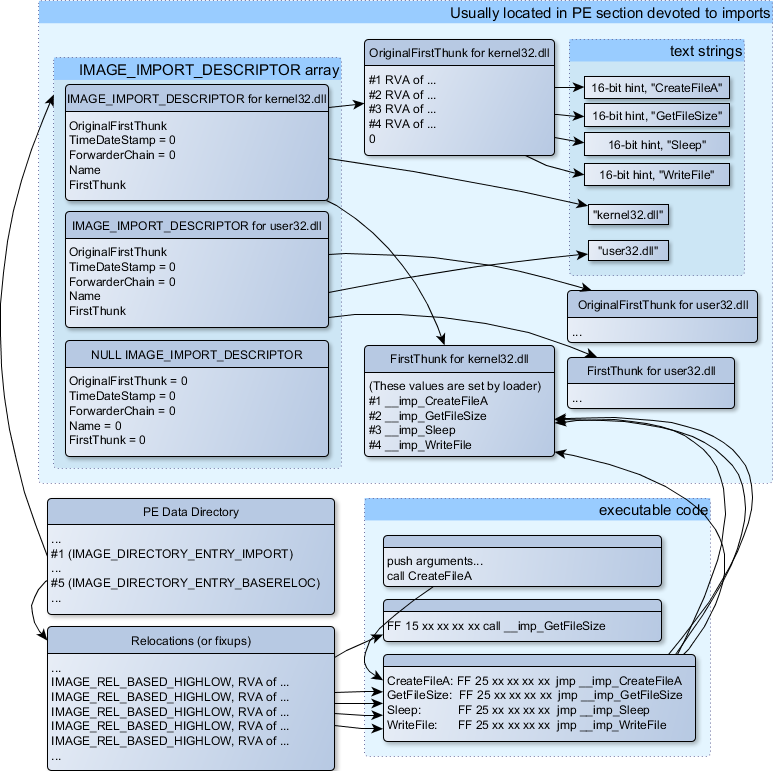
\includegraphics[scale=\FigScale]{OS/PE/unnamed0.png}
\caption{\RU{схема, объединяющая все структуры в PE-файлы, связанные с импортами}
\EN{A scheme that unites all PE-file structures related to imports}}
\end{figure}

\RU{Самая главная структура\EMDASH{}это массив}\EN{The main structure is the array} \IT{IMAGE\_IMPORT\_DESCRIPTOR}.
\RU{Каждый элемент на каждую импортируемую DLL}\EN{Each element for each DLL being imported}.

\RU{У каждого элемента есть}\EN{Each element holds the} \ac{RVA}\RU{-адрес}\EN{ address} 
\RU{текстовой строки (имя DLL)}\EN{of the text string (DLL name)} (\IT{Name}).

\IT{OriginalFirstThink} \RU{это}\EN{is the} \ac{RVA} \RU{-адрес таблицы \ac{INT}}\EN{address of the \ac{INT} table}. 
\RU{Это массив}\EN{This is an array of} 
\ac{RVA}\RU{-адресов}\EN{ addresses},
\RU{каждый из которых указывает на текстовую строку где записано имя функции}
\EN{each of which points to a text string with a function name}. 
\RU{Каждую строку предваряет 16-битное число}\EN{Each string is prefixed by a 16-bit integer} 
(\q{hint})\EMDASH\RU{\q{ординал} функции}\EN{\q{ordinal} of function}.

\RU{Если при загрузке удается найти функцию по ординалу, тогда сравнение текстовых строк не будет происходить.
Массив оканчивается нулем.}
\EN{While loading, if it is possible to find a function by ordinal,
then the strings comparison will not occur. The array is terminated by zero.}
\RU{Есть также указатель на таблицу \ac{IAT} с названием}
\EN{There is also a pointer to the \ac{IAT} table named} \IT{FirstThunk},
\RU{это просто}\EN{it is just the} \ac{RVA}\RU{-адрес}\EN{ address} 
\RU{места, где загрузчик будет проставлять адреса найденных функций}\EN{of the place where the loader
writes the addresses of the resolved functions}.

\RU{Места где загрузчик проставляет адреса, \IDA именует их так}
\EN{The points where the loader writes addresses are marked by \IDA like this}: \IT{\_\_imp\_CreateFileA}, \etc{}.

\RU{Есть по крайней мере два способа использовать адреса, проставленные загрузчиком}
\EN{There are at least two ways to use the addresses written by the loader}.

\begin{itemize}
\index{x86!\Instructions!CALL}
\item
\RU{В коде будут просто инструкции вроде}\EN{The code will have instructions like} 
\IT{call \_\_imp\_CreateFileA}, 
\RU{а так как, поле с адресом импортируемой функции это как бы глобальная переменная}
\EN{and since the field with the address of the imported function is a global variable in some sense}, 
\RU{то в таблице релоков добавляется адрес (плюс 1 или 2) в инструкции \IT{call}}
\EN{the address of the \IT{call} instruction (plus 1 or 2) is to be added to the relocs table},
\RU{на случай если модуль будет загружен по другому базовому адресу}
\EN{for the case when the module is loaded at a different base address}.

\RU{Но как видно, это приводит к увеличению таблицы релоков}\EN{But, obviously, this may enlarge
relocs table significantly}.
\RU{Ведь вызовов импортируемой функции у вас в модуле может быть очень много}
\EN{Because there are might be a lot of calls to imported functions in the module}.
\RU{К тому же, чем больше таблица релоков, тем дольше загрузка}
\EN{Furthermore, large relocs table slows down the process of loading modules}.

\index{x86!\Instructions!JMP}
\index{thunk-\RU{функции}\EN{functions}}
\item
\RU{На каждую импортируемую функцию выделяется только один переход на импортируемую функцию используя
инструкцию \JMP плюс релок на эту инструкцию}
\EN{For each imported function, there is only one jump allocated, using the \JMP instruction 
plus a reloc to it}.
\RU{Такие места-\q{переходники} называются также \q{thunk}-ами}\EN{Such points are also called \q{thunks}}.
\RU{А все вызовы импортируемой функции это просто инструкция \CALL на соответствующий \q{thunk}}
\EN{All calls to the imported functions are just \CALL instructions to the corresponding \q{thunk}}.
\RU{В данном случае, дополнительные релоки не нужны, потому что эти CALL-ы имеют относительный адрес,
и корректировать их не надо}\EN{In this case, additional relocs are not necessary because these CALL-s
have relative addresses and do not need to be corrected}.
\end{itemize}

\RU{Оба этих два метода могут комбинироваться}\EN{These two methods can be combined}.
\RU{Вероятно, линкер создает отдельный \q{thunk}, если вызовов слишком много, но по умолчанию\EMDASH{}не создает.}
\EN{Possible, the linker creates individual \q{thunk}s if there are too many calls to the function,
but not done by default.} \\
\\
\RU{Кстати, массив адресов функций, на который указывает FirstThunk,
не обязательно может быть в секции \ac{IAT}}\EN{By the way, the array of function addresses to which FirstThunk is
pointing is not necessary to be located in the \ac{IAT} section}.
\RU{К примеру, автор сих строк написал утилиту}\EN{For example, author of these lines once wrote the}
PE\_add\_import\footnote{\href{http://go.yurichev.com/17049}{yurichev.com}} 
\RU{для добавления импорта в уже существующий .exe-файл}\EN{utility for adding imports to an existing .exe-file}.
\RU{Раньше, в прошлых версиях утилиты, на месте функции, вместо которой вы хотите подставить вызов в другую DLL,
моя утилита вписывала такой код:}
\EN{Some time earlier, in the previous versions of the utility, 
at the place of the function you want to substitute with a call to another DLL,
my utility wrote the following code:}

\begin{lstlisting}
MOV EAX, [yourdll.dll!function]
JMP EAX
\end{lstlisting}

\RU{При этом, FirstThunk указывает прямо на первую инструкцию.
Иными словами, загрузчик, загружая yourdll.dll, 
прописывает адрес функции \IT{function} прямо в коде.}
\EN{FirstThunk points to the first instruction. In other words, when loading yourdll.dll,
the loader writes the address of the \IT{function} function right in the code.}

\RU{Надо также отметить что обычно секция кода защищена от записи}
\EN{It also worth noting that a
code section is usually write-protected}, \RU{так что, моя утилита
добавляет флаг}\EN{so my utility adds the} \\
\IT{IMAGE\_SCN\_MEM\_WRITE} 
\RU{для секции кода. Иначе при загрузке такой программы, она упадет с ошибкой}
\EN{flag for code section. Otherwise, the program to crash while loading with error code}
5 (access denied). \\
\\
\RU{Может возникнуть вопрос: а что если я поставляю программу с набором DLL,
которые никогда не будут меняться (в т.ч., адреса всех функций в этих DLL), может как-то можно ускорить процесс загрузки?}
\EN{One might ask: what if I supply a program with a set of DLL files which is not supposed to change (including addresses of all DLL functions),
is it possible to speed up the loading process?}

\RU{Да, можно прописать адреса импортируемых функций в массивы FirstThunk заранее}
\EN{Yes, it is possible to write the addresses of the functions to be imported into the FirstThunk arrays in advance}.
\RU{Для этого в структуре}\EN{The \IT{Timestamp} field is present in the} \\
\IT{IMAGE\_IMPORT\_DESCRIPTOR} \RU{имеется поле \IT{Timestamp}}\EN{structure}.
\RU{И если там присутствует какое-то значение, то загрузчик сверяет это значение с датой-временем DLL-файла}
\EN{If a value is present there, then the loader compares this value with the date-time of the DLL file}.
\RU{И если они равны, то загрузчик больше ничего не делает, и загрузка может происходить быстрее.}
\EN{If the values are equal, then the loader does not do anything, and the loading of the process can be faster.}
\RU{Это называется}\EN{This is called} \q{old-style binding}
\footnote{\href{http://go.yurichev.com/17050}{MSDN}.
\RU{Существует также}\EN{There is also the} \q{new-style binding}.}.
\index{BIND.EXE}
\RU{В Windows SDK для этого имеется утилита BIND.EXE}
\EN{The BIND.EXE utility in Windows SDK is for for this}.
\RU{Для ускорения загрузки вашей программы}\EN{For speeding up the loading of your program}, 
Matt Pietrek \InENRU \cite{Pietrek1}, \RU{предлагает делать binding сразу после инсталляции
вашей программы на компьютере конечного пользователя}\EN{suggests to do the binding shortly after your program
installation on the computer of the end user}. \\
\\
\RU{Запаковщики/зашифровщики PE-файлов могут также сжимать/шифровать таблицу импортов}
\EN{PE-files packers/encryptors may also compress/encrypt imports table}.
\RU{В этом случае, загрузчик Windows, конечно же, не загрузит все нужные DLL}
\EN{In this case, the Windows loader, of course, will not load all necessary DLLs}.
\index{Windows!Win32!LoadLibrary}
\index{Windows!Win32!GetProcAddress}
\RU{Поэтому распаковщик/расшифровщик делает это сам, при помощи вызовов}
\EN{Therefore, the packer/encryptor does this on its own, with the help of} 
\IT{LoadLibrary()} \AndENRU \EN{the }\IT{GetProcAddress()}\EN{ functions}.
\RU{Вот почему в запакованных файлах эти две функции часто присутствуют в \ac{IAT}.}
\EN{That is why these two functions are often present in \ac{IAT} in packed files.}\\
\\
\RU{В стандартных DLL входящих в состав Windows, часто, \ac{IAT} находится в самом начале PE-файла.}
\EN{In the standard DLLs from the Windows installation, \ac{IAT} often is located right in the beginning of the PE file.}
\RU{Возможно это для оптимизации}\EN{Supposedly, it is done for optimization}.
\RU{Ведь .exe-файл при загрузке не загружается в память весь 
(вспомните что инсталляторы огромного размера подозрительно быстро запускаются), он \q{мапится} (map), 
и подгружается в память частями по мере обращения к этой памяти.}
\EN{While loading, the .exe file is not loaded into memory as a whole (recall huge install programs which are
started suspiciously fast), it is \q{mapped}, and loaded into memory in parts as they are accessed.}
\RU{И возможно в Microsoft решили что так будет быстрее.}
\EN{Probably, Microsoft developers decided it will be faster.}

\subsection{\RU{Ресурсы}\EN{Resources}}

\label{PEresources}
\RU{Ресурсы в PE-файле\EMDASH{}это набор иконок, картинок, текстовых строк, описаний диалогов}
\EN{Resources in a PE file are just a set of icons, pictures, text strings, dialog descriptions}.
\RU{Возможно, их в свое время решили отделить от основного кода, чтобы все эти вещи были многоязычными,
и было проще выбирать текст или картинку того языка, который установлен в \ac{OS}}
\EN{Perhaps, they were separated from the main code, so all these things could be multilingual,
and it would be simpler to pick text or picture for the language that is currently set in the \ac{OS}}. \\
\\
\RU{В качестве побочного эффекта, их легко редактировать и сохранять обратно в исполняемый файл,
даже не обладая специальными знаниями, например, редактором ResHack}%
\EN{As a side effect, they can be edited easily and saved back to the executable file, even if one does not have special knowledge, 
by using the ResHack editor, for example} (\myref{ResHack}).

\subsection{.NET}

\index{.NET}
\RU{Программы на .NET компилируются не в машинный код, а в свой собственный байткод}
\EN{.NET programs are not compiled into machine code but into a special bytecode}.
\index{OEP}
\RU{Собственно, в .exe-файлы байткод вместо обычного кода, однако, точка входа (\ac{OEP}) 
указывает на крохотный фрагмент x86-кода}\EN{Strictly speaking, there is bytecode instead of the usual x86 code
in the .exe file, however, the entry point (\ac{OEP}) points to this tiny fragment of x86 code}:

\begin{lstlisting}
jmp         mscoree.dll!_CorExeMain
\end{lstlisting}

\RU{А в mscoree.dll и находится .NET-загрузчик, который уже сам будет работать с PE-файлом.}
\EN{The .NET loader is located in mscoree.dll, which processes the PE file.}
\index{Windows!Windows XP}
\RU{Так было в \ac{OS} до Windows XP. Начиная с XP, загрузчик \ac{OS} уже сам определяет, что это
.NET-файл и запускает его не исполняя этой инструкции \JMP}
\EN{It was so in all pre-Windows XP \ac{OS}es. Starting from XP, the \ac{OS} loader is able to detect the .NET file
and run it without executing that \JMP instruction}
\footnote{\href{http://go.yurichev.com/17051}{MSDN}}.

\index{TLS}
\subsection{TLS}

\RU{Эта секция содержит в себе инициализированные данные для}\EN{This section holds initialized
data for the} \ac{TLS}(\myref{TLS}) (\RU{если нужно}\EN{if needed}).
\RU{При старте нового треда, его}\EN{When a new thread start, its} 
\ac{TLS}\RU{-данные инициализируются данными из этой секции}
\EN{data is initialized using the data from this section}. \\
\\
\index{TLS!Callbacks}
\RU{Помимо всего прочего, спецификация PE-файла предусматривает инициализацию}
\EN{Aside from that, the PE file specification also provides initialization of the}
\ac{TLS}\RU{-секции, т.н.,}\EN{ section, the so-called} TLS callbacks.
\RU{Если они присутствуют, то они будут вызваны перед тем как передать управление на главную точку входа}
\EN{If they are present, they are to be called before the control is passed to the main entry point} (\ac{OEP}).
\RU{Это широко используется запаковщиками/защифровщиками PE-файлов.}
\EN{This is used widely in the PE file packers/encryptors.}

\subsection{\RU{Инструменты}\EN{Tools}}

\begin{itemize}
\item
\index{objdump}
\index{Cygwin}
objdump (\RU{имеется в}\EN{present in} cygwin) \RU{для вывода всех структур PE-файла}\EN{for dumping all PE-file structures}.

\item
\index{Hiew}
Hiew(\myref{Hiew}) \RU{как редактор}\EN{as editor}.

\item
	pefile\EMDASH{}Python-\RU{библиотека для работы с PE-файлами}\EN{library for PE-file processing}
\footnote{\url{http://go.yurichev.com/17052}}.

\item
\label{ResHack}
ResHack \acs{AKA} Resource Hacker\EMDASH{}\RU{редактор ресурсов}\EN{resources editor}
\footnote{\url{http://go.yurichev.com/17052}}.

\item
	PE\_add\_import\footnote{\url{http://go.yurichev.com/17049}}\EMDASH{}
\RU{простая утилита для добавления символа/-ов в таблицу импортов PE-файла}
\EN{simple tool for adding symbol(s) to PE executable import table}.

\item
	PE\_patcher\footnote{\href{http://go.yurichev.com/17054}{yurichev.com}}\EMDASH{} 
\RU{простая утилита для модификации PE-файлов}\EN{simple tool for patching PE executables}.

\item
	PE\_search\_str\_refs\footnote{\href{http://go.yurichev.com/17055}{yurichev.com}}\EMDASH{} 
\RU{простая утилита для поиска функции в PE-файле, где используется некая текстовая строка}
\EN{simple tool for searching for a function in PE executables which use some text string}.
\end{itemize}

\subsection{Further reading}

% FIXME: bibliography per chapter or section
\begin{itemize}
\item
Daniel Pistelli\EMDASH{}The .NET File Format \footnote{\url{http://go.yurichev.com/17056}}
\end{itemize}

